\documentclass[11pt]{amsart}

% Standard letter size paper with 1inch margins
\usepackage[letterpaper, margin=1in]{geometry}

% Useful packages 
\usepackage{amsmath, amssymb, amsthm, amsaddr}
\usepackage{enumerate, subcaption, graphicx, hyperref}
\usepackage{algorithm}
\usepackage{algpseudocode}
\usepackage{cite}
\usepackage{titling}
\usepackage{bm}

% Custom math commands
\newcommand{\I}{\mathrm{i}}
\DeclareMathOperator{\E}{e}

\title{HMS 581 Final Project}
\newcommand{\subtitle}{\large Modeling Measles in New York \& Vermont}
\author{Hunter Lybbert}
\address{Applied Mathematics Department, University of Washington, Seattle, WA 
\\ \texttt{hlybbert@uw.edu}}
\date{\today}

\pretitle{\begin{center}\LARGE}
\posttitle{\par\medskip\subtitle\end{center}}
\preauthor{\begin{center}
\normalsize \lineskip 0.5em
\begin{tabular}[t]{c}}
\postauthor{\end{tabular}\end{center}}
\predate{\begin{center}\small}
\postdate{\end{center}}

\begin{document}

\begin{center}
    {\LARGE \textbf{HMS 581 Final Project}}\\[1ex]
    {\large Modeling Measles in New York \& Vermont}\\[4ex]
    {\Large Hunter Lybbert}\\[2ex]
    \textit{Applied Mathematics Department, University of Washington, Seattle, WA}\\[1ex]
    \texttt{hlybbert@uw.edu}\\[1ex]
    \today
\end{center}

\vspace{2ex}
\begin{quote}
A\textsc{bstract.}
\small We model the spread of the measles pathogen in New York and Vermont from January 1$^{\text{st}}$, 1930 to January 1$^{\text{st}}$, 1940 using an SIR model.
Our model has been augmented from a basic SIR model to incorporate annual seasonality, births and deaths, and a multi-year seasonality term for the strength of the strain of the pathogen.
To optimize and fit our model, we adapted to python, the R implementation of particle MCMC provided to us.
\end{quote}

\section{Introduction and Model Augmentations}\label{sec:augmentations}
The standard SIR model tracks the portion of or total number of people from the population which are susceptible, infectious, and recovered.
Our model has been augmented with parameters accounting for annual seasonality, births and deaths, and a multi year oscillating strength of the strain of the pathogen. The basic model is given by
\begin{align*}
\frac{dS}{dt} &= \sigma N - \beta I \frac S N - \mu S \\
\frac{dI}{dt} &= \beta I \frac S N - \gamma I - \mu I \\
\frac{dR}{dt} &= \gamma I - \mu R.
\end{align*}
\subsection{Seasonality} This one is a no brainer to add to the model because like the common flu we are familiar with measles has a higher transmission rate in certain parts of the year.
\subsection{Birth Deaths}
I attempted to fit the model with a separate parameter for birth $\sigma$ and death $\mu$ but this did not do any better than just using $\mu$ as these equations are usually presented.
Additionally, I tried to choose intelligent initial guesses such as the known births divided by known population in the initial year 1930.
\subsection{Pathogen Strength (Multi-year oscilations)} In Figure \ref{fig:f1} we see the observed cases for our years of interest.
Notice that in addition to the obvious annual seasonality there appears to also be a process of some kind governing just how strong the peak is for each year.
This is the behavior I wanted to capture with the multi-year pathogen strain strength oscillations.
However, I was unable to implement this in the time I had for this assignment.
This was due to the fact that I spent too much time getting pMCMC to work in python.
And then tried to get something working on the smaller number of parameters without the pathogen strength.

\section{Model Fitting and Results}\label{sec:results}
I chose to fit the model using pMCMC as implemented in class, however adapted to work in python.
The fitting process did not go as well as we hoped.
Often times the results were extremely sensitive to the standard deviations used in the proposal distribution draws as well as the initial guess.
We also tried letting it run for many more pMCMC steps, without any better luck.
See Figure \ref{fig:f2} for a sample plot of the parameters moving about in one of the pMCMC fits.
Additionally, Figure \ref{fig:f3} shows one of the best fits we could get given the time we had to spend on the project thus far.

\begin{figure}[h]
	\centering
	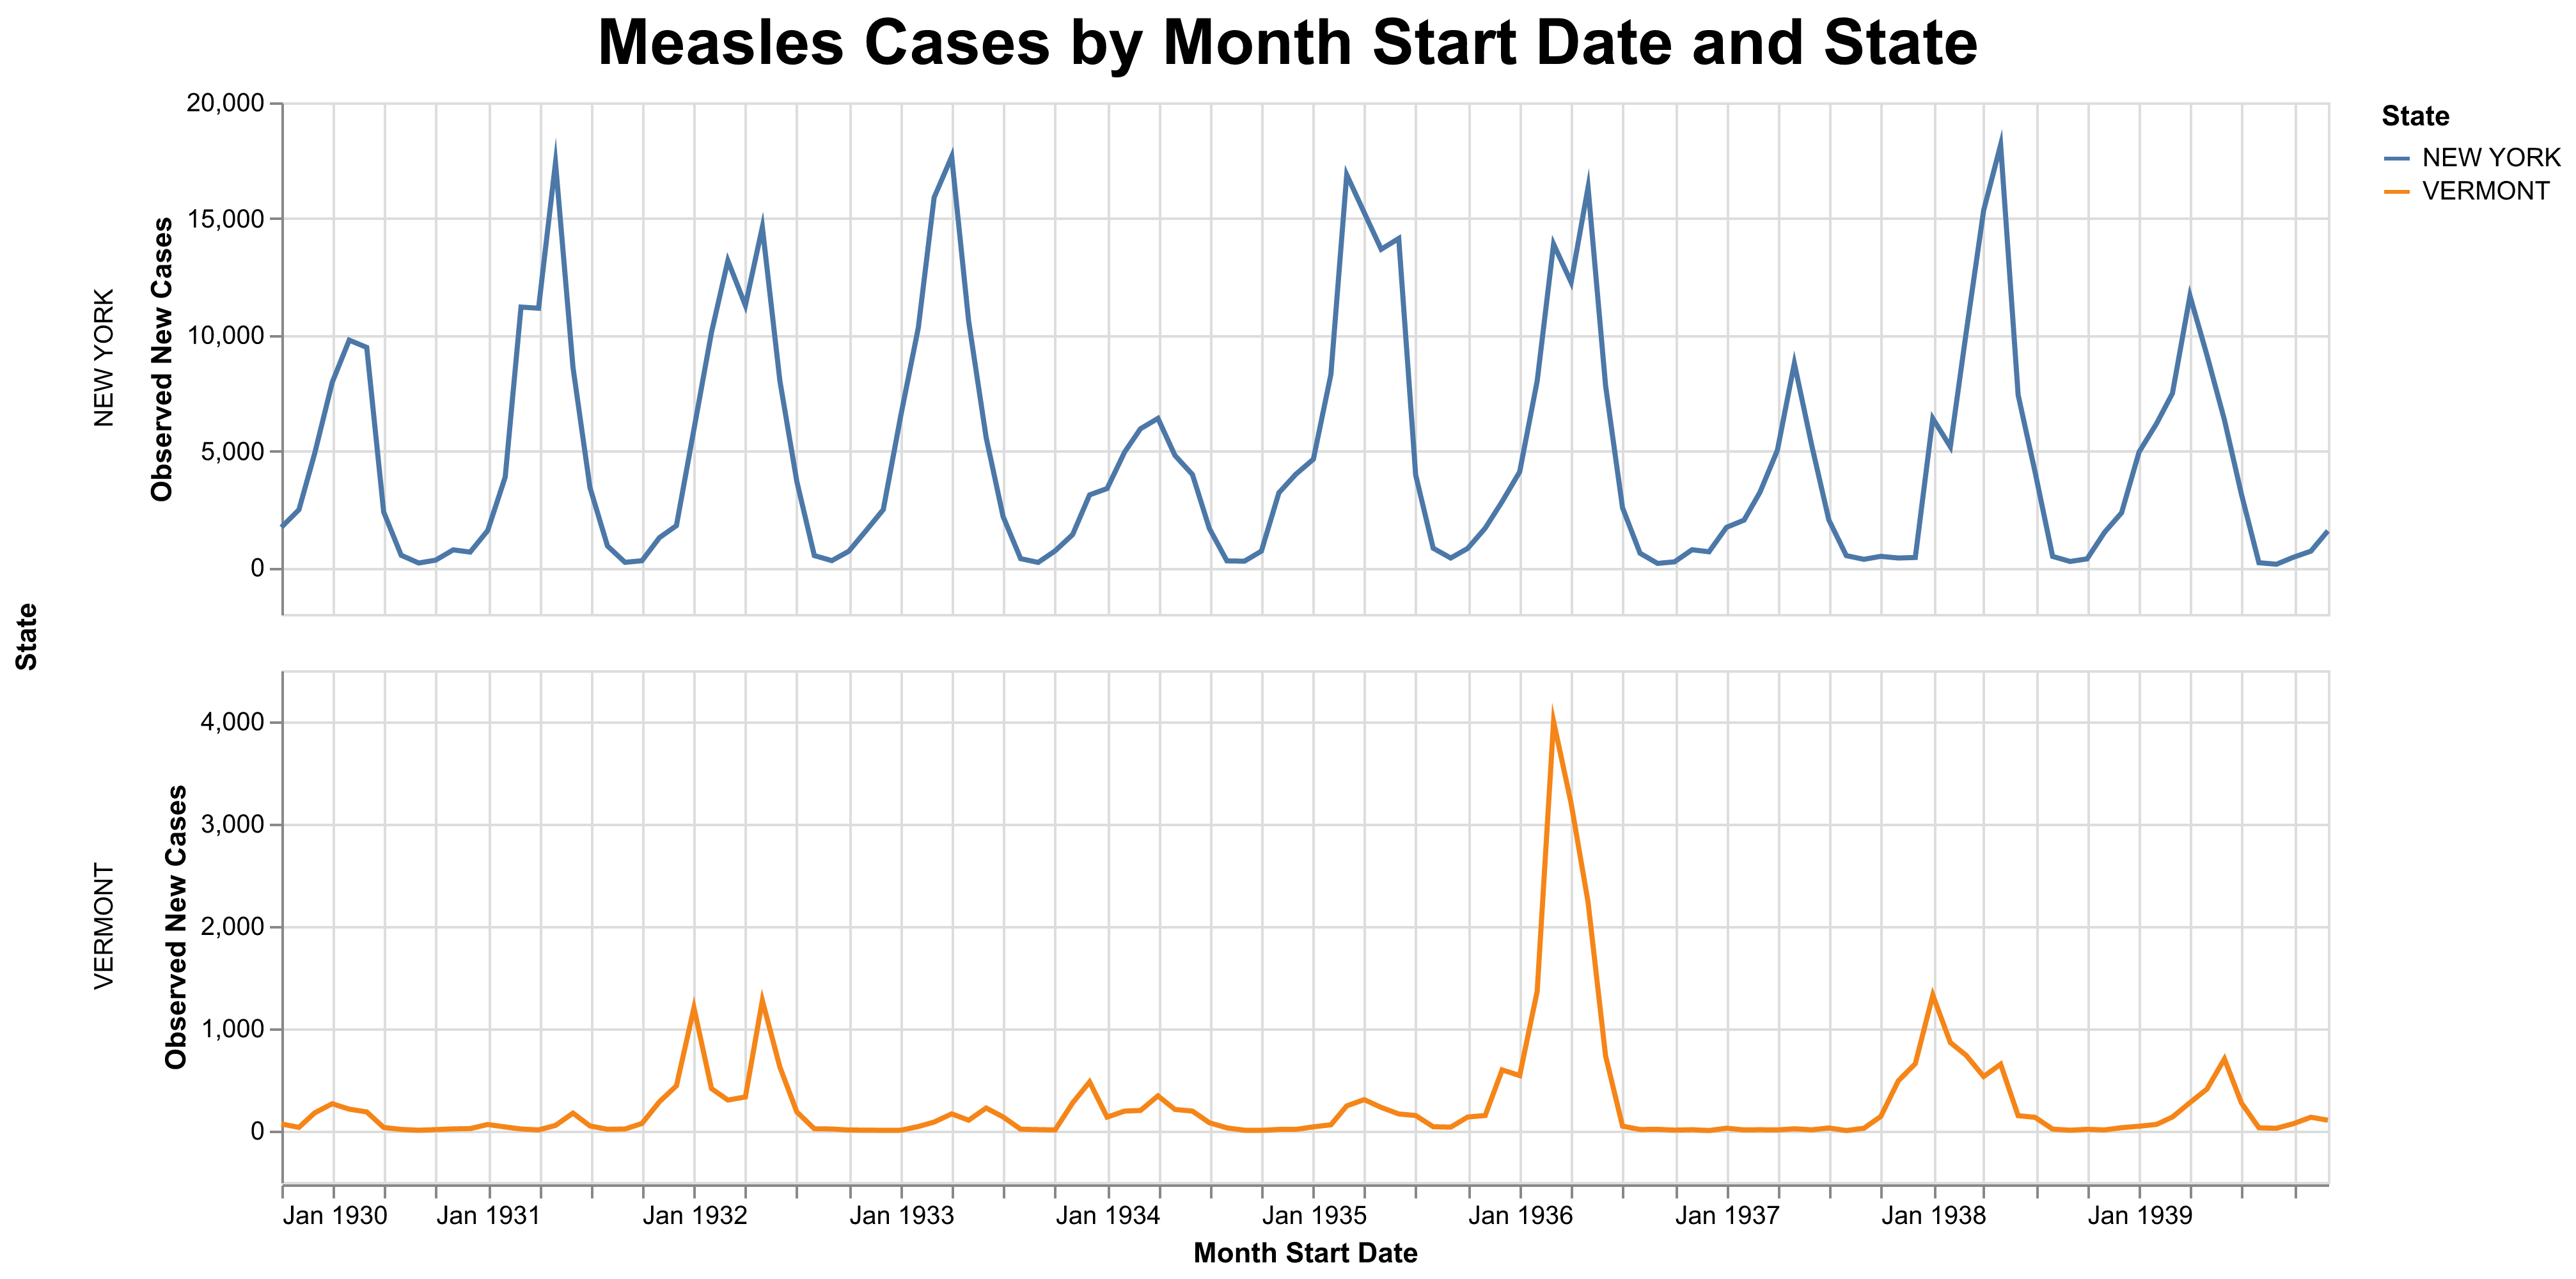
\includegraphics[width=1\textwidth]{../visuals/measles_cases_by_state_and_month_start.png}
 	\caption{The observed cases per month from 1930 to end of 1939 for both New York and Vermont.}\label{fig:f1}
\end{figure}

\begin{figure}[h]
	\centering
	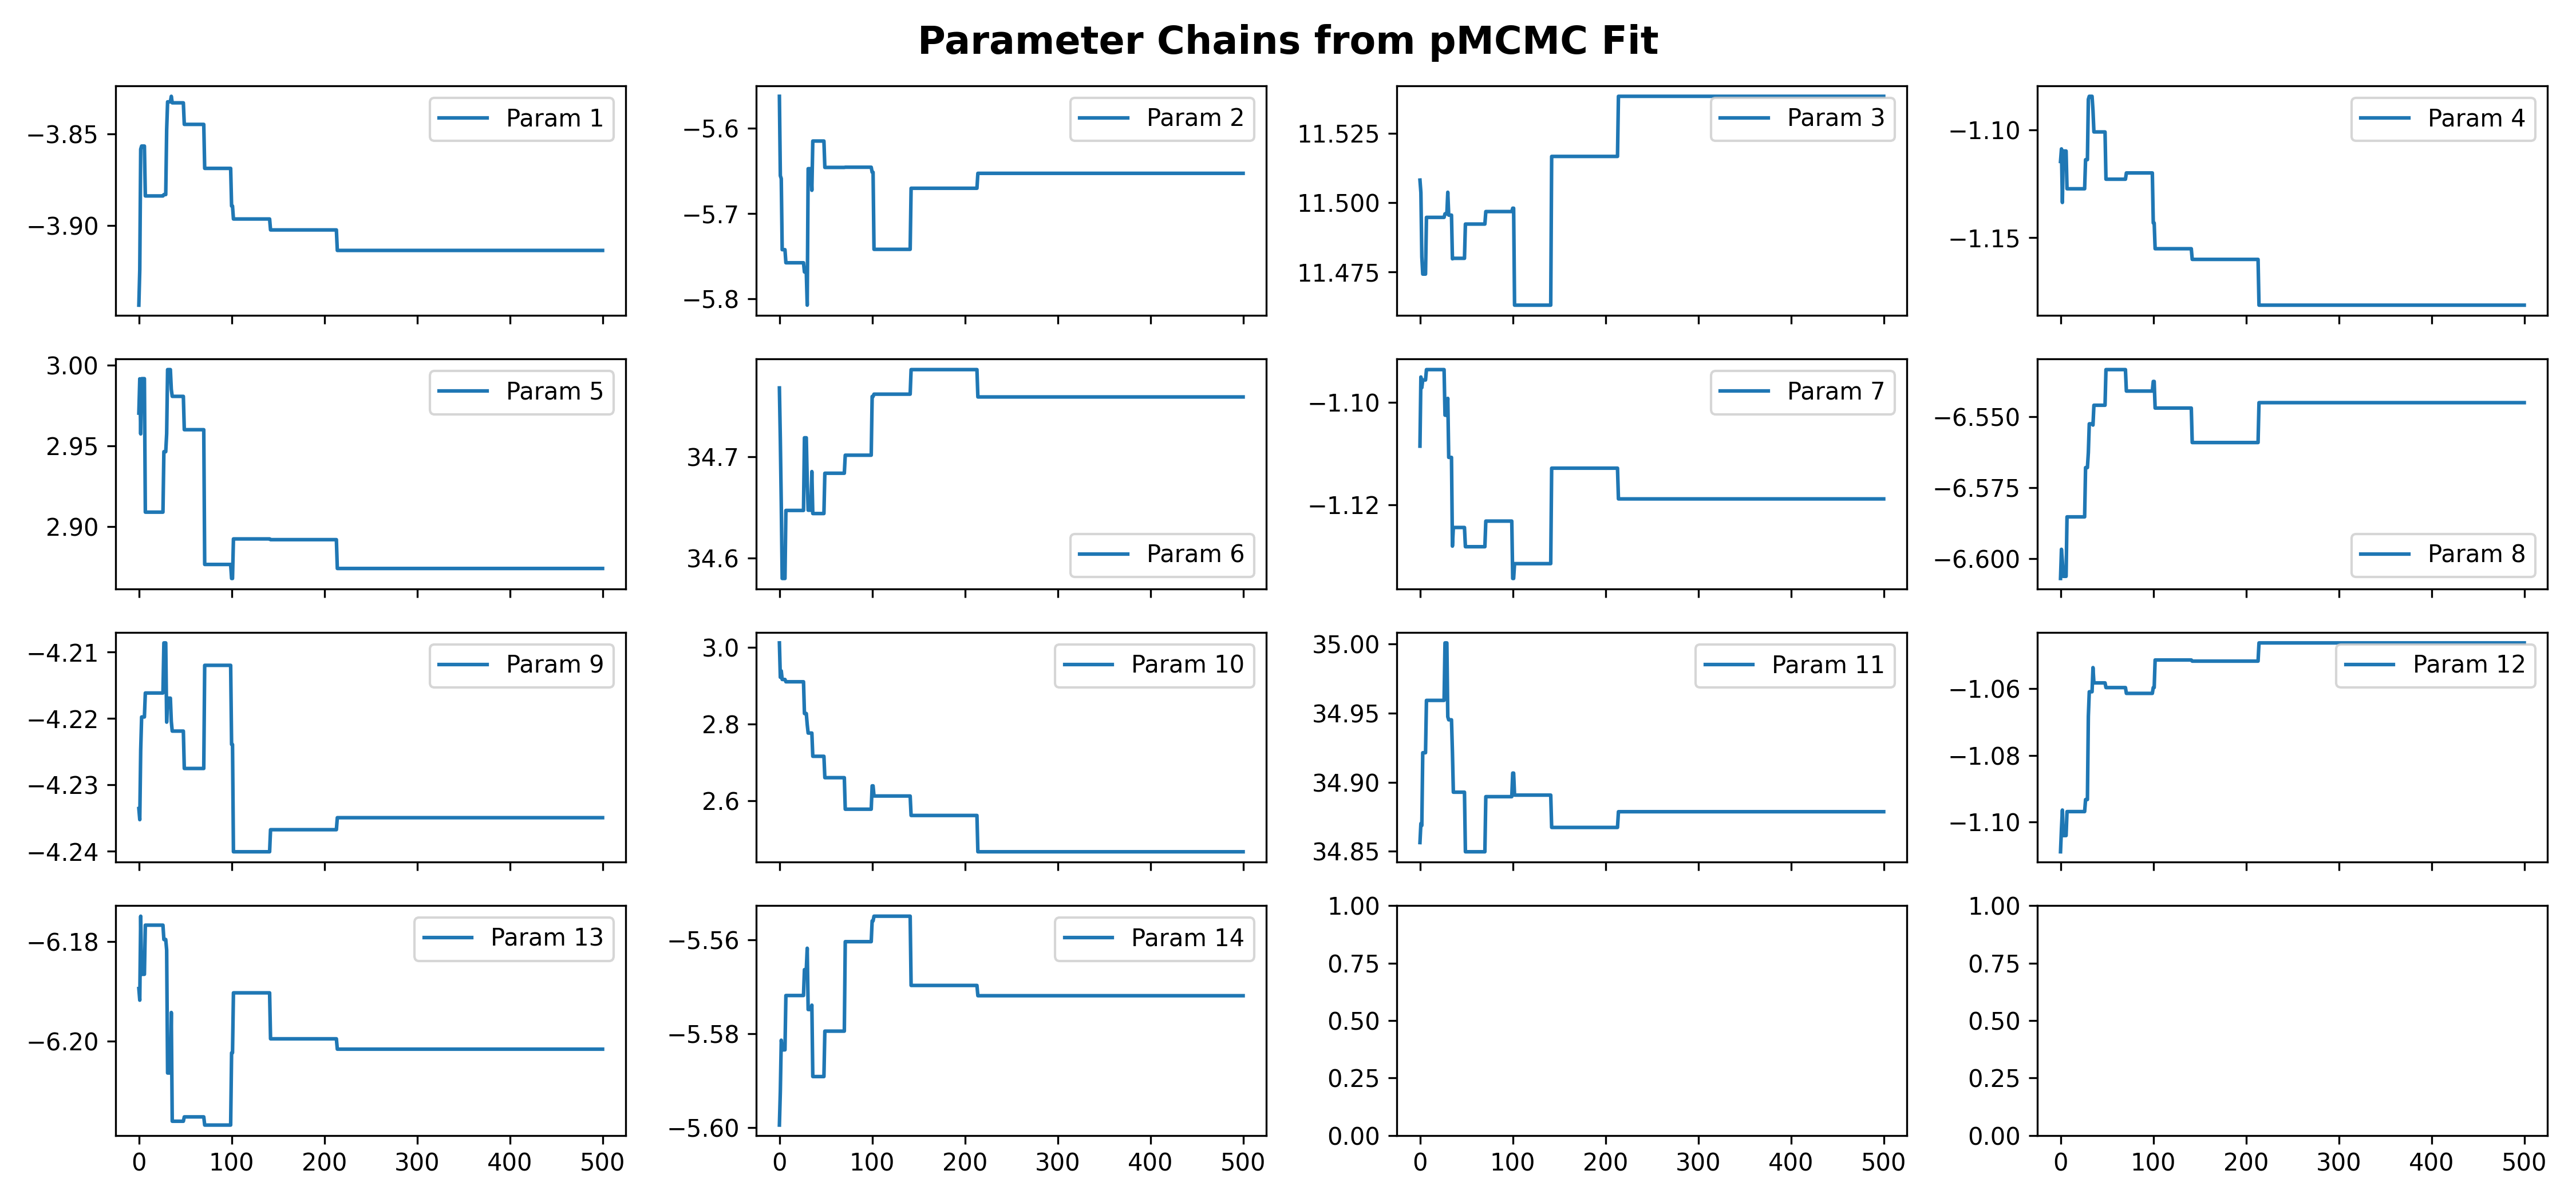
\includegraphics[width=1\textwidth]{../visuals/pmcmc_parameter_chains.png}
 	\caption{The values of each parameter over the 500 pMCMC steps.}\label{fig:f2}
\end{figure}

\begin{figure}[h]
	\centering
	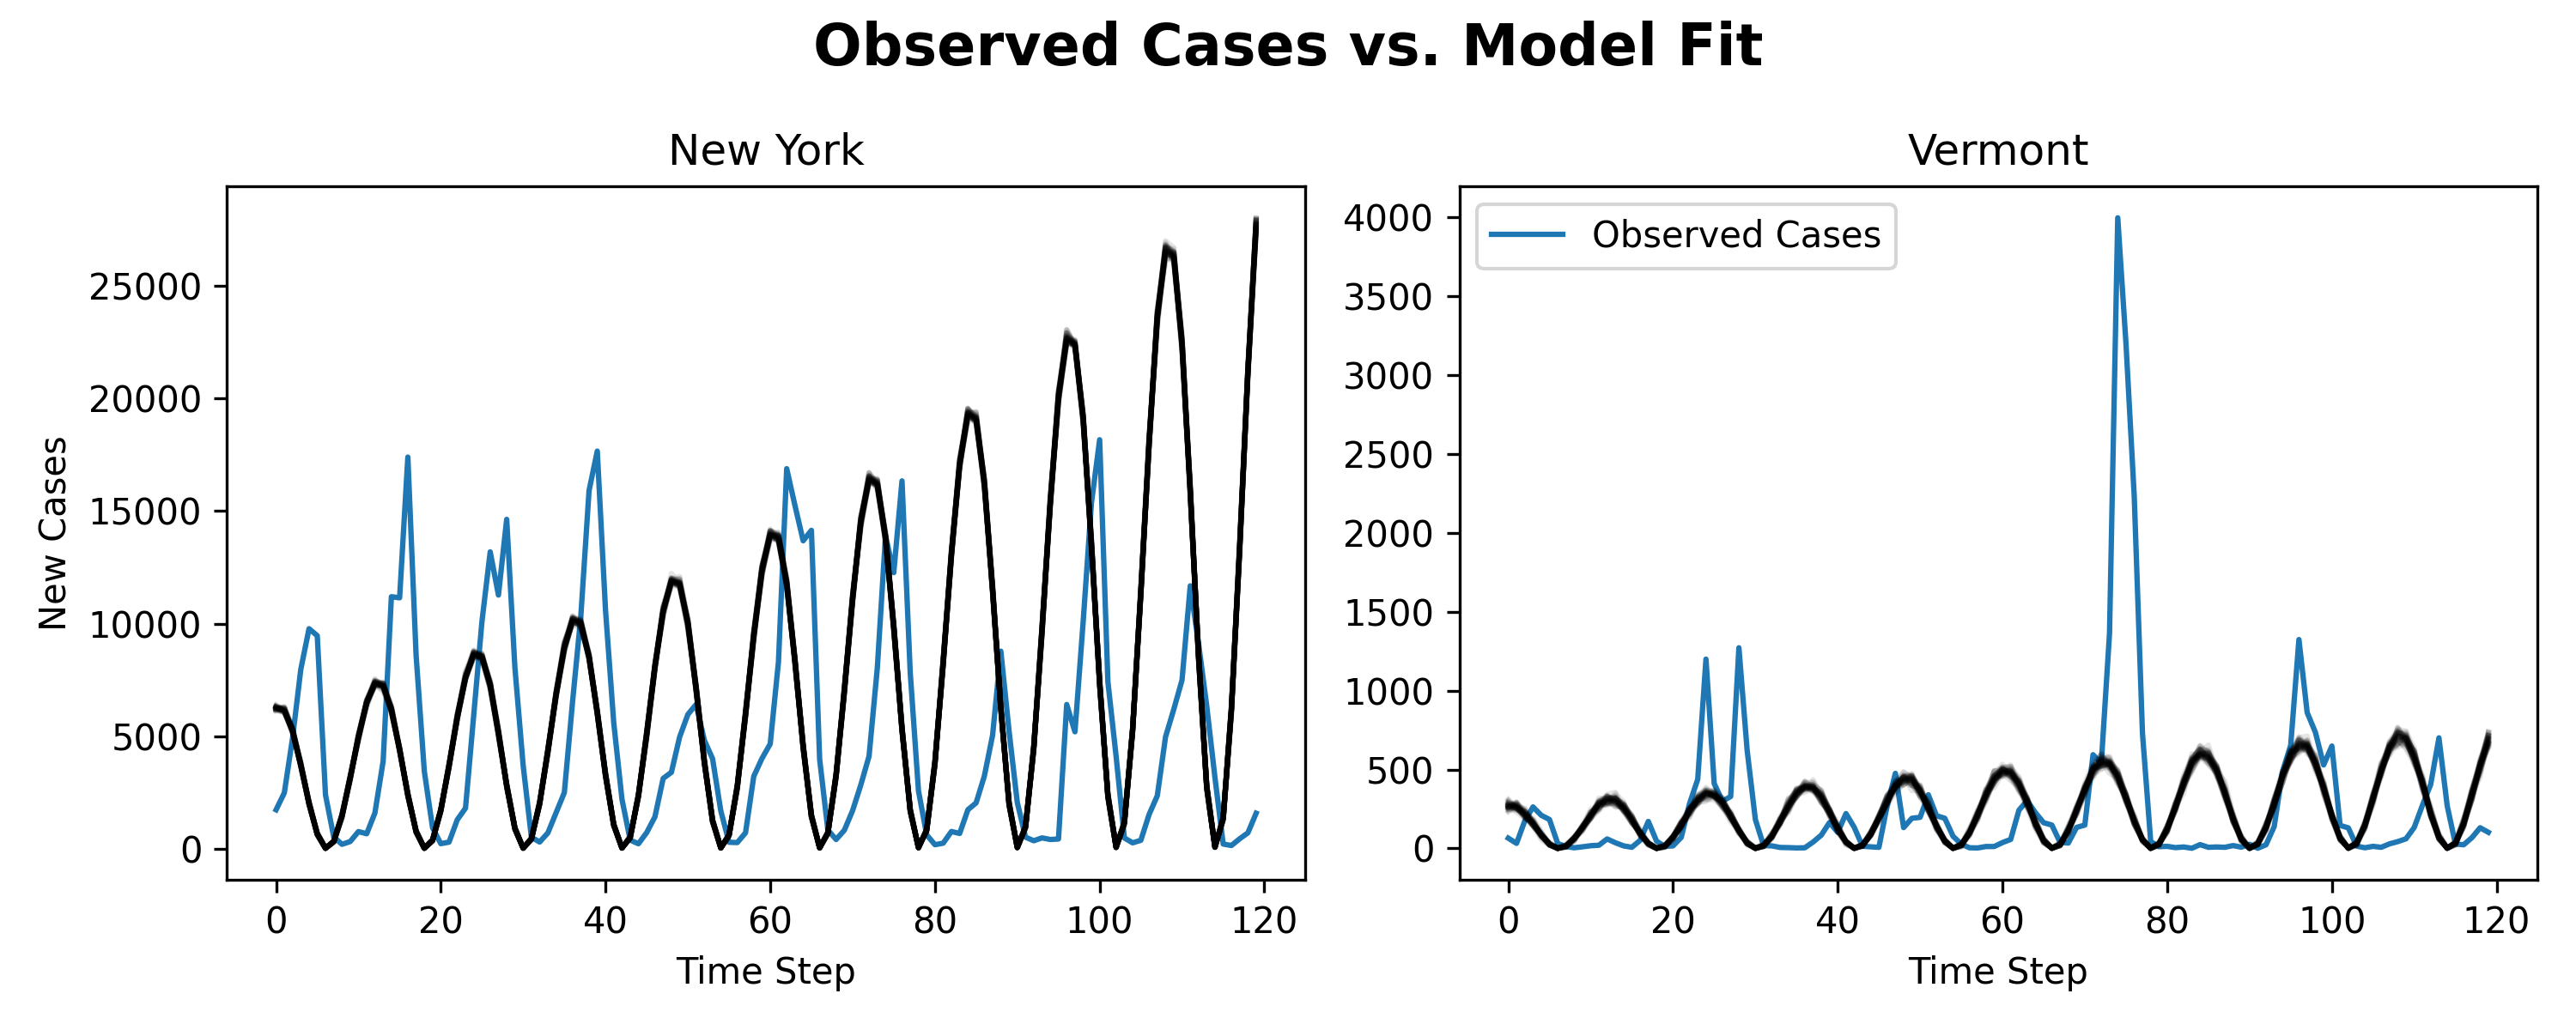
\includegraphics[width=1\textwidth]{../visuals/measles_ny_vt_obs_cases_model_fit.png}
 	\caption{Observed cases versus the fitted model new cases for both New York and Vermont.}\label{fig:f3}
\end{figure}

\section{Conclusion}\label{sec:conclustion}
One of the biggest challenges was determining good initial guess for the parameters and determining the best standard deviations to use in the proposal distribution while performing pMCMC.
Our fit was not exceptionally good and I would not have trusted it as a tool to forecast future spread of the measles pathogen.
Additional augmentations that we could use to further improve the model (though the issues with initial guess and proposal distribution in pMCMC would need to be resolved first for these to help) include migration between states and actually implement the pathogen strain strength.

\section*{Acknowledgements}
We would like to thank Bobby Reiner for a very instructive course and giving us ample opportunities to apply the material we learned in the classroom.
We would like to acknowledge the assistants from Nate Ward, Jaxon Tuggle, and Hailey Sparks who were instrumental in brainstorming ideas, debugging code, and analyzing results together.

\newpage
\appendix

\section{Best Fit Statistics}
These are the resulting parameters after fitting the model with pMCMC.
\begin{table}[h]
    \centering
    \begin{tabular}{|c|l|l|} % 'l' for left-aligned, 'c' for center-aligned columns
        \hline
        \textbf{Param} & \textbf{Value} & \textbf{Description} \\ 
        \hline
        $\beta$ & 0.01997 & Rate of transmission \\
        \hline
        $\gamma$ & 0.00351 & Recovery rate \\
	\hline
        season & 0.99999 & The peak strength of the rate of transmission \\
        \hline
        peak & 2.81781 & The month where the peak strength of rate of transmission occurs \\
        \hline
        $S_0$ (NY) & 0.94655 & Initial fraction of New York pop. that is susceptible \\
        \hline
        $I_0$ (NY) & 0.27958 & Initial fraction of New York pop. that is infected \\
        \hline
        $\rho$ (NY) & 0.24622 & Rate that the new infections are reported at \\
        \hline
        $\sigma$ (NY) & 0.00144 & Birth rate in New York \\
        \hline
        $\mu$ (NY) & 0.01448 & Death rate in New York \\
        \hline
        $S_0$ (VT) & 0.92183 & Initial fraction of Vermont pop. that is susceptible \\
        \hline
        $I_0$ (VT) & 0.28459 & Initial fraction of Vermont pop. that is infected \\
        \hline
        $\rho$ (VT) & 0.25994 & Rate that the new infections are reported at \\
        \hline
        $\sigma$ (VT) & 0.00203 & Birth rate in Vermont \\
        \hline
        $\mu$ (VT) & 0.0038 & Death rate in Vermont \\
        \hline
    \end{tabular}
    \caption{This is the set of best parameters using pMCMC found for fitting our model.
    The model represented in Figure \ref{fig:f3} was produced by these parameters.}
    \label{tab:tab0}
\vspace*{-1mm}
\end{table}

\section{Code}
The code can be found on \href{https://github.com/hunter-lybbert/uw-central/tree/main/disease_dynamics/final_project}{GitHub}.

\end{document}
